\subsection{Numerical Experiments}

In this section we elaborate on our synthetic setting and provide evidence for admissability of our method in comparison to the naive method.
Our codes can be found at \href{https://github.com/scO0rpion/Fields-Experiment-Project}{https://github.com/scO0rpion/Fields-Experiment-Project}.

\begin{figure}[h!]
    \centering
    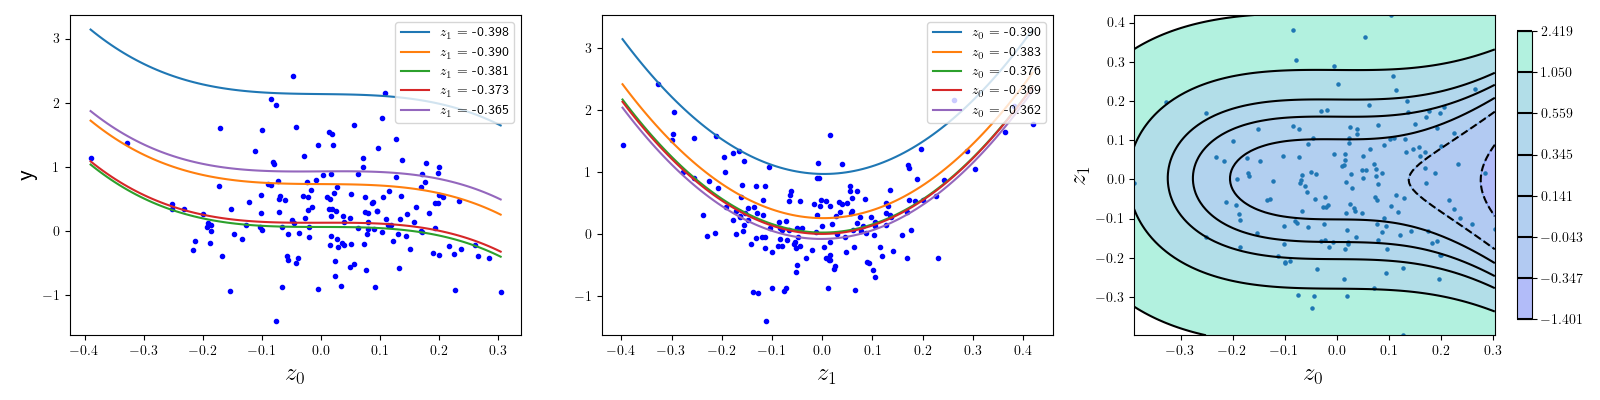
\includegraphics[width=\textwidth]{regression_fcn.png}
    \caption{Demonstrates the regression function $f_e(z_0, z_1)$ for a particular environment. The dots correspond to latent data points $(Z^{e}_i, Y^{e}_i)$ projected onto the underlying central subspace, i.e. $Z^{e}_i = B^{\T} X^{e}_i$. (left) The lines correspond to the graph of $z_0 \mapsto f(z_0,z_1)$ for different values of $z_1$. 
    (middle) The lines correspond to the graph of $z_1 \mapsto f(z_0,z_1)$ for different values of $z_0$.
    (right) The contour plot of the regression function $f_e$.}
\end{figure}

\begin{figure}[h!]
    \label{fig:singular}
    \centering
    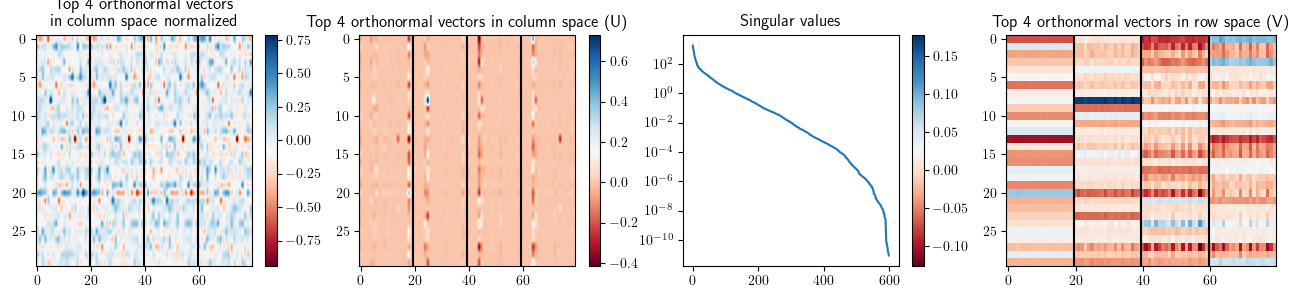
\includegraphics[width=\textwidth]{svd.png}
    \caption{An illustration of singular value decomposition of $M^{\environments \times \environments} = U^{\environments} \Lambda {V^{\environments}}^{\T}$. Top 4 singular vectors separated by black lines. Each singular vector $U^{\environments}_i \in \mathbb{R}^{dT}$ is reshaped into matrix in $\mathbb{R}^{d \times T}$ where $e$'th column represents $U_i^e$.
    (left) Each column is normalized to have length one. (left middle) Vectors in column space of $M^{\environments \times \environments}$. (right midle) Singular values demonstrate a sharp decay verifying $M^{\environments \times \environments}$ is of low rank. (right) Vectors in row space of $M^{\environments \times \environments}$. }
\end{figure}

Recall that our goal in this paper is to accurately recover the invariant central subspace using datasets from different environments. 
We generate our central subspace unfiromly at random among $k=2$ dimenional subspaces in $\mathbb{R}^{d}$ with ambient dimension $d = 30$, i.e. $\mathscr{L} = \col(B)$ where entries of $B \in \mathbb{R}^{d \times k}$ are generated from standard gaussian. 
Note that we assume the knowledge of the instrinsic dimension $k$ throughout. This value can also be estimated based on how fast the singular values of $M^{\environments \times \environments}$ drops (see Figure \ref{fig:singular}). 
We generate $T = 20$ environments for which their corresponding distribution $\probability[e]$ is obtained in the following way:
\begin{enumerate}
    \item \textbf{Random Design:} The covariates follows anisotropic gaussian $X^{e} \sim \mathcal{N}(0, \fracl{\Sigma^e}{\sqrt{d}})$ where $\Sigma^e$ is diagonal with diagonal elements following standard chi distribution.
    Similar results can be obtained when the covariates are isotropic. 
    \item \textbf{Polynomial Regression Function:} We consider a polynomial regression function with random coefficient generated from standard cauchy,
    $$ f_e(z) = a_0^e z_0^4 + a_1^e z_1^2 + a_2^e z_0 z_1$$
    \item \textbf{Homogenous Noise:} Our response variable is obtained as $Y^e = f_e(B^{\T} X^{e}) + \epsilon^e$ where the noise is gaussian with variance $\sigma = 0.5$.
\end{enumerate}
We generate datasets $\dataset[e]$ with $n$ samples from each environment and fit a regression function estimator $\hat{f}_e$ using kernel regression with a RBF kernel. Additionally we perform a 80-20 percent sample splitting to tune the hyperparameters.
Finally, we evaluate the performance of our algorithm averaged over 20 experiments for each choice of sample size $n$ and demonstrate the results in Figure~\ref{fig:results}.

